
\section{Study Dataset}

We select the simulation results and validation analysis done by \citet{Taborda_2014_BSSA} as our reference dataset. In that study, the authors carried out deterministic simulations for the 2008 \eqmag{w} 5.4 Chino Hills, California, earthquake using a finite-element approach. The simulations, done for a kinematic finite-fault model of the earthquake, were computed for a maximum frequency \fmaxeq{4} and a minimum shear wave velocity \vsmineq{200}. In total, \citet{Taborda_2014_BSSA} did three simulations, each for a different velocity model \citep[CVM-S4, CVM-H, CVM-H+GTL, see][]{Small_2017_SRL}. The modeling domain covered an area of \adomain{180}{135}{km} that included all the major sedimentary basins and other relevant geologic structures in the greater Los Angeles region. Their validation analysis consisted of comparisons with data recorded during the event at 336 ground motion monitoring stations, for the three component of motion (EW, NS, and UD). The simulation domain and the stations used for the analysis are shown in Figure \ref{fig:chino-hills}, and the validation results obtained by \citet{Taborda_2014_BSSA} for the GOF analysis of the broadband signals using \citeauthor{Anderson_2004_Proc}'s approach is shown in Figure \ref{fig:ref-gof-maps} for the three simulation sets.

\begin{figure*}
    \centering
    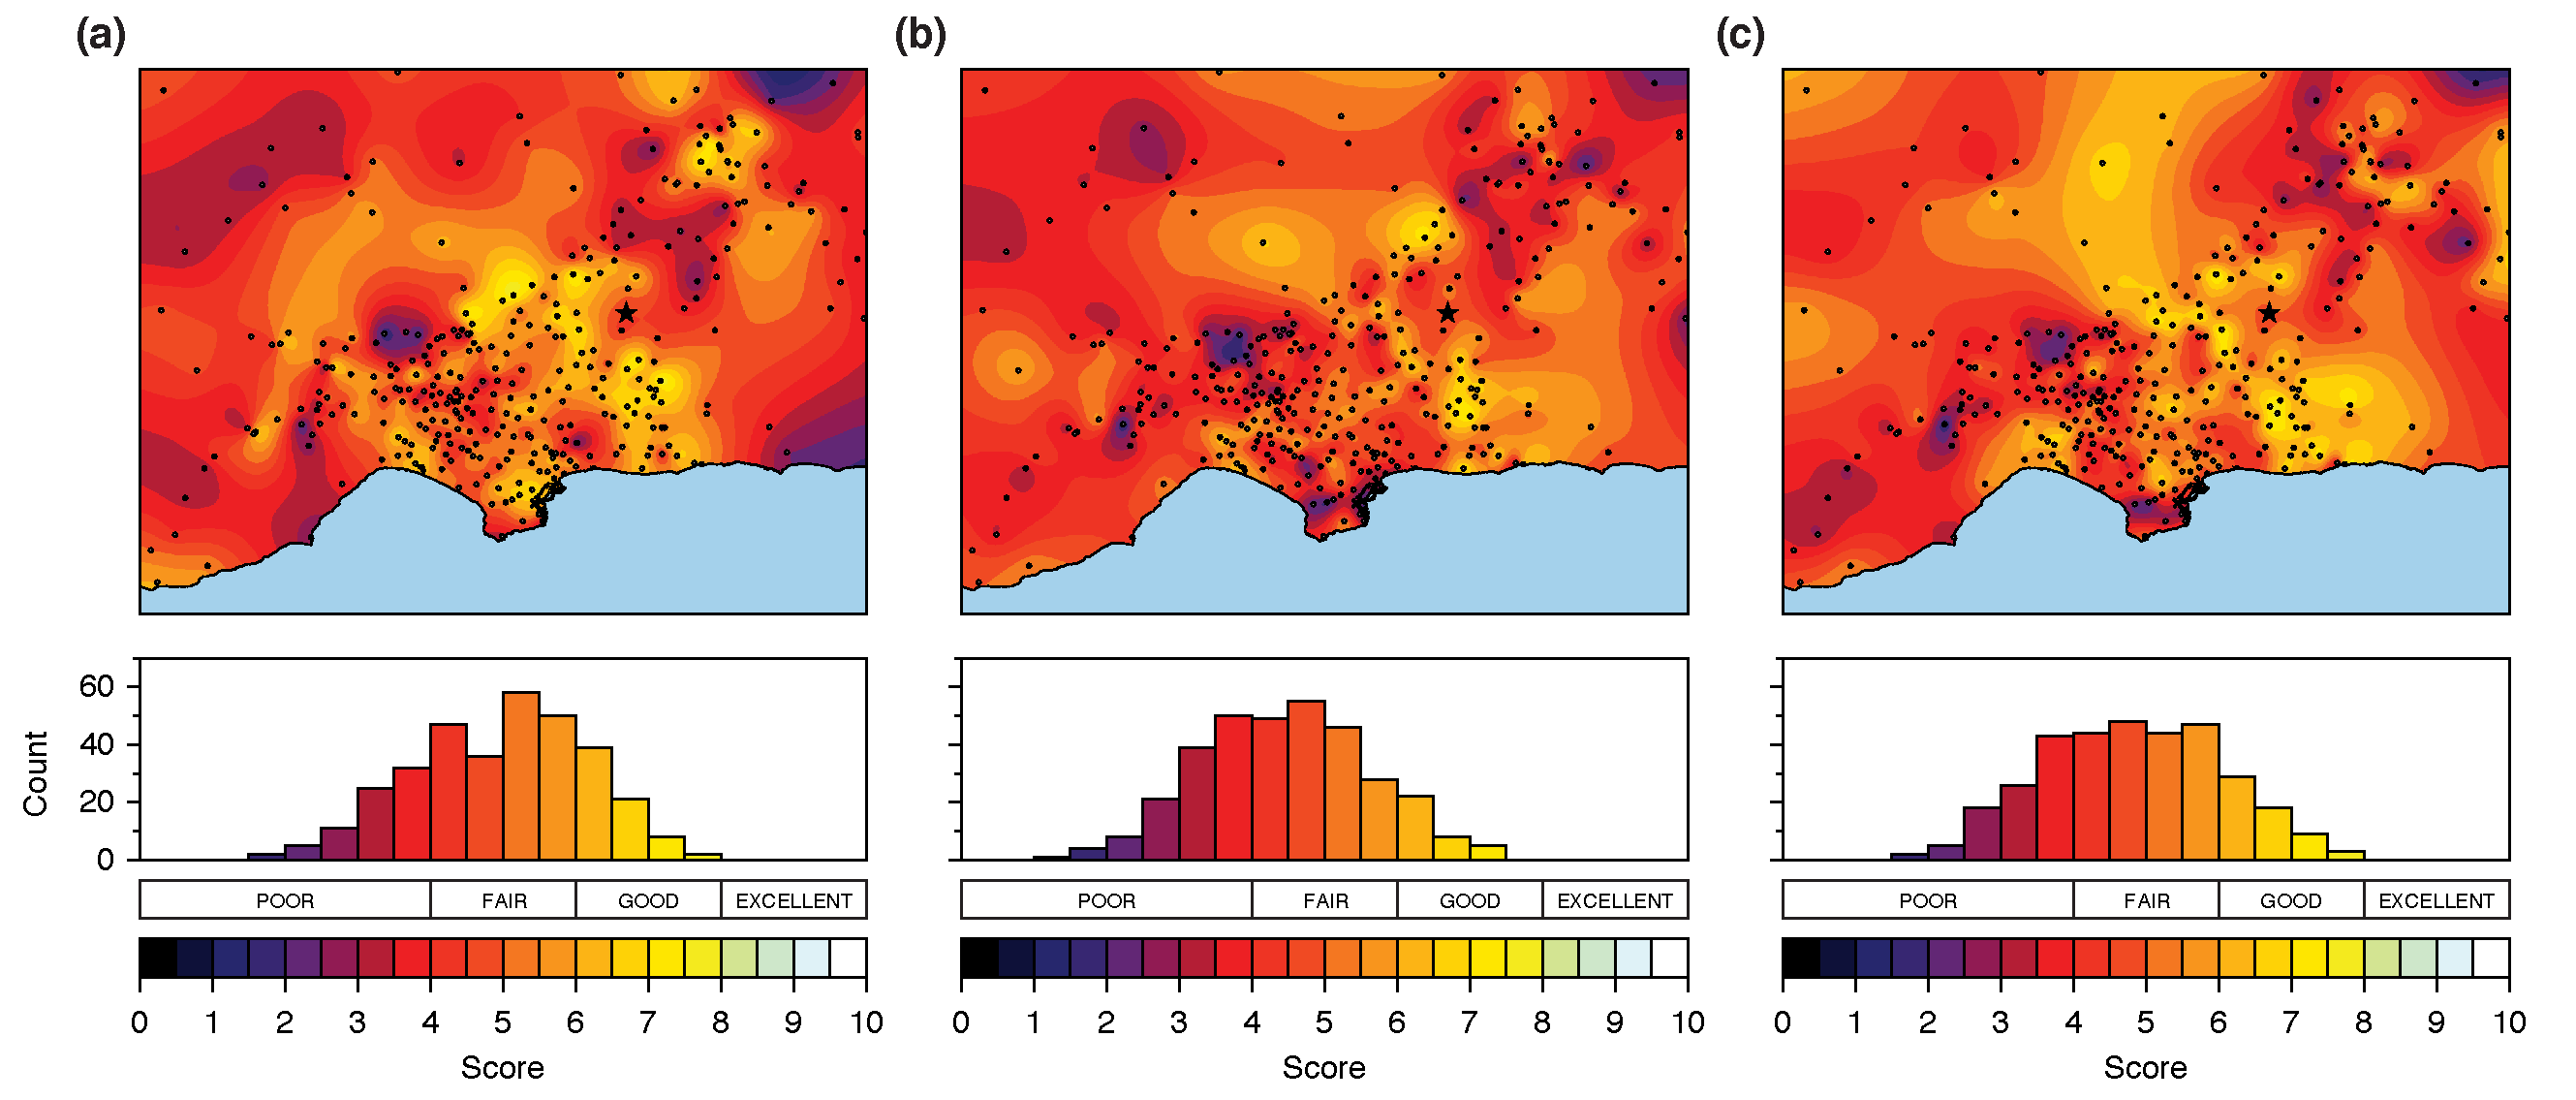
\includegraphics[width=\textwidth]{figures/pdf/figure-02}
    \caption{Validation results obtained by \citet{Taborda_2014_BSSA} in the form of GOF values across the region of interest obtained from comparisons between simulations for three different velocity models and data recorded at ground motion monitoring stations.}
    \label{fig:ref-gof-maps}
\end{figure*}

Here, we use the GOF scores obtained by \citet{Taborda_2014_BSSA} independently of the velocity models and/or the component of motions. Although at times we will make distinctions between the models and the components for visualization purposes, the clustering analysis to be described in the following section was done using the whole dataset of scores. The motivation behind this choice was that the dataset, as a sample of GOF values, was independent of the simulation and serves here as a generic set for the purpose of identifying the correlations that exist between the different metrics in Table \ref{tab:metrics}. As such, given the simulations for each velocity model (3), the motion components (3), and the number of stations used in the validation (336) gave us a large enough sample of 3,024 GOF scores. Figure \ref{fig:data-box-plot} illustrates this idea by comparing the statistical distribution of the broadband GOF scores of the simulations classified by velocity models and components. It is clear that although there are differences between them, these are negligible; in other words, the statistical distribution of results for each metric is about the same independently of model or component.

\begin{figure}
    \centering
    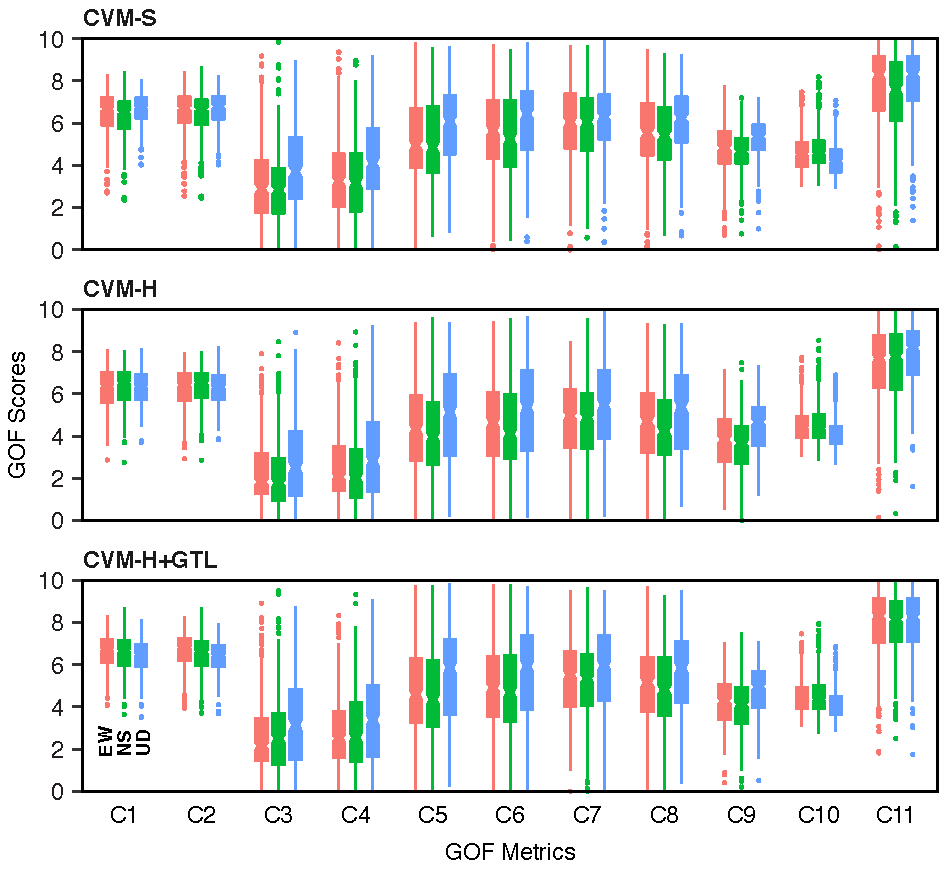
\includegraphics[width=\columnwidth]{figures/pdf/figure-03}
    \caption{Statistical distribution of the GOF scores used in this study based on the validation results obtained by \citet{Taborda_2014_BSSA} shown in the form of box-plots for each metric (C1 through C11, see Table \ref{tab:metrics}), velocity model (CVM-S, CVM-H, and CVM-H+GTL), and component of motion (NS, EW, UD). In each case, the median is indicated by a notch in the box of the central quartiles, and the lines represent the interquartile range (Q3-Q1), with outliers shown as scattered dots.}
    \label{fig:data-box-plot}
\end{figure}

% ===========================================================================================
%
% OLD NAEEM VERSION
% 
% State of California is an earthquake prone region with a long history of seismicity. The Los Aneles basin, due to its unique geologic sediments, has been studied from different perspective. Numerous high resolution velocity models are developed mainly to conduct forward ground motion simulation. Occurrence of frequent moderate magnitude earthquakes made the Los Angeles basin as a natural laboratory for seismic  studies specially testing the forward ground motion simulation modeling. In a relatively recent study, \citet{Taborda_2014_BSSA} conducted a comprehensive study in order to assess the functionality of developed velocity models in the Los Angeles basin and surrounding areas. They simulated the 2008 Chino Hills earthquake using 3 velocity models including: CVM-S4, CVM-H, and CVM-H+GTL (for more details about these models see \citet{Taborda_2014_BSSA}.)
% They computed the GOF scores based on \citet{Anderson_2004_Proc}, with minor modification introduced by \citet{Taborda_2013_BSSA} as discussed in the validation section. Fig.~\ref{fig:epicenters} shows the location of the epicenter and seismic stations. 

% \begin{figure}
%     \centering
%     \includegraphics
%        % [width=\columnwidth]
%         [width=450px]
%         {figures/pdf/Figure_1}
%     \caption{(a) Region of interest and epicentral location of the 2008 $M_W ~ 5.4$ Chino Hills earthquake (highlighted). Focal mechanism is shown at the margin of the region of interest. Major quaternary faults in the area are shown in the back along with the main roads and county divisions. (b) Simulation area of interest. Dots indicate the location of the 336 stations considered in this study for validation. The main local and interstate roads are also shown here. In both panels, the background shows the hillshade topography of the region. The color version of this figure is available only in the electronic edition.}
%     \label{fig:epicenters}
% \end{figure}

% We use \citet{Taborda_2014_BSSA} database where they computed 11 scores for 3 different velocity models. In this study we only analyze the results for broadband which in this case is \feq{0.1}{4}. Fig.~\ref{fig:data_box_plot} shows the box plot of all data that we used in this study which we separate them in velocity models and components. In total we use $336 \times 3 \times 3 = 3024$ individual pair of data and synthetic.

% \begin{figure}
%     \centering
%     \includegraphics
%        % [width=\columnwidth]
%         [width=\textwidth]
%         {figures/pdf/Figure_2.pdf}
%     \caption{Box plot of data used in the study. Metrics are shown for C1 to C11 for 3 components and in separate plots for velocity models. Median of data are shown as a notch. Thick lines represent the IQR (Interquartile Range, Q3-Q1) of data. Outliers (data less than Q1-1.5*IQR and greater than Q3+1.5*IQR) are shown as scatter dots above and below plots if applicable.}
%     \label{fig:data_box_plot}
% \end{figure}

% As we explained before, we use all data set regardless of velocity models and components. However, distinguishing data for velocity model and components can answer the question that if the goodness of fit scores dependent on them. Addressing this research question is beyond the scope of this paper. We distinguish data based on velocity models and components only in presenting data or results.   

% Fig.~\ref{fig:data_density}  shows the density distribution of each score for CVM-S. The figure shows the variation of different metrics with components. Except in cross correlation (C10) in all metrics the up-down (UD) component scores are about the same or higher than horizontal components. 

% \begin{figure}
%     \centering
%     \includegraphics
%        % [width=\columnwidth]
%         [width=\textwidth]
%         {figures/pdf/Figure_3.pdf}
%     \caption{Distribution of data (only CVM-S) for different components in different scores based on different components. Each distribution has a unit area.}
%     \label{fig:data_density}
% \end{figure}






